\subsection{Perawatan Aplikasi}

\begin{frame}{Koreksi Daftar $C_p$ Airfoil}
  Melalui penggunaan variabel $C_p$ terhadap koordinat yang tepat agar \textit{looping} berjalan baik\footnote{\url{https://github.com/akbarpn136/aerofoil/commit/23e88ea0a61c71c6a33d930979cf7119a0944173}}.

  \begin{columns}[t]
    \begin{column}{.5\linewidth}
      \begin{figure}[h]
        \centering
        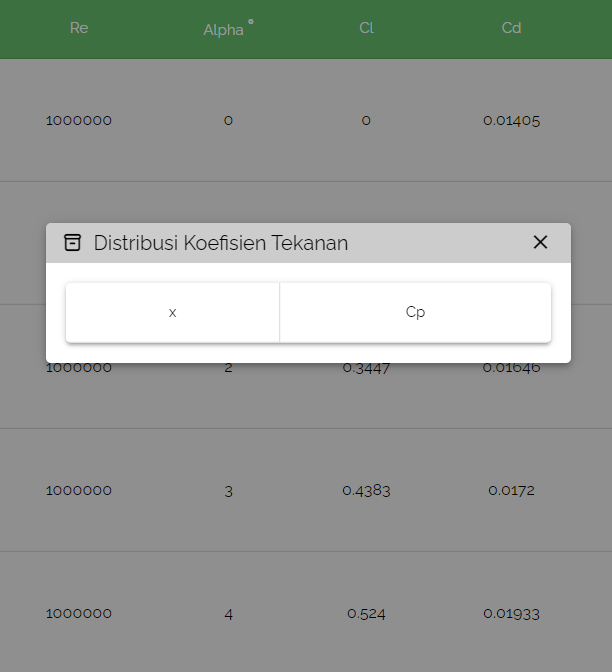
\includegraphics[width=0.4\linewidth]{statics/fix_bug_cpx}
        \caption{Sebelum koreksi}
      \end{figure}
    \end{column}

    \begin{column}{.5\linewidth}
      \begin{figure}[h]
        \centering
        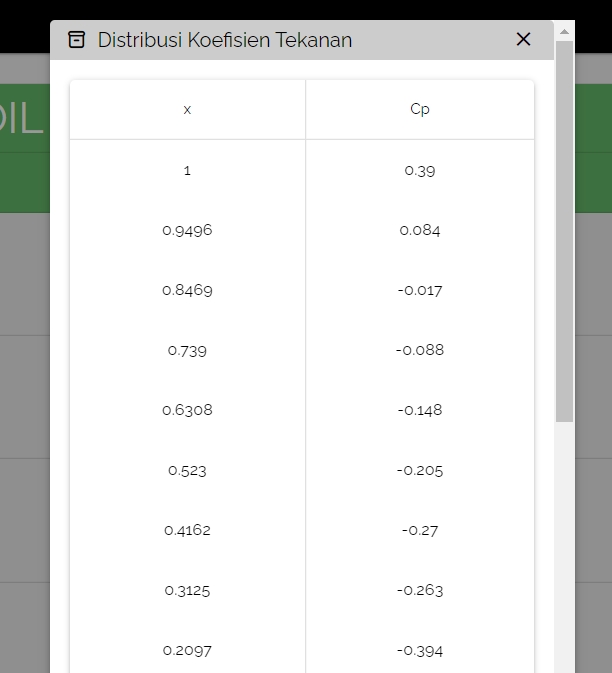
\includegraphics[width=0.4\linewidth]{statics/result_cpx}
        \caption{Setelah koreksi}
      \end{figure}
    \end{column}
  \end{columns}
\end{frame}

\begin{frame}{Koreksi Kualitas Airfoil}
  Kualitas citra airfoil ditingkatkan lagi agar kualitas SDF juga lebih baik\footnote{\url{https://github.com/akbarpn136/aerofoil/commit/f20639a210a27dbcdd9aabcf3cf07b2ca2223d0d}}.

  \pause

  \begin{columns}[t]
    \begin{column}{.25\linewidth}
      \begin{figure}[h]
        \centering
        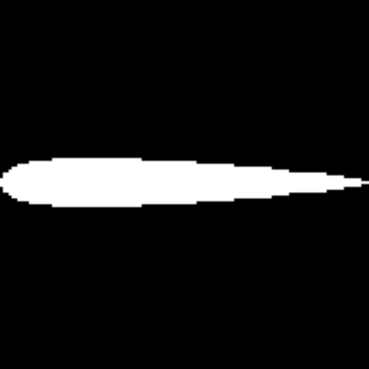
\includegraphics[width=0.8\linewidth]{statics/airfoil_low.png}
        \caption{Biner low}
      \end{figure}
    \end{column}

    \begin{column}{.25\linewidth}
      \begin{figure}[h]
        \centering
        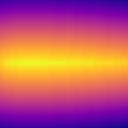
\includegraphics[width=0.8\linewidth]{statics/airfoil_sdf_low.png}
        \caption{SDF low}
      \end{figure}
    \end{column}

    \begin{column}{.25\linewidth}
      \begin{figure}[h]
        \centering
        
\includegraphics[width=0.8\linewidth]{statics/airfoil_high.png}
        \caption{Biner high}
      \end{figure}
    \end{column}

    \begin{column}{.25\linewidth}
      \begin{figure}[h]
        \centering
        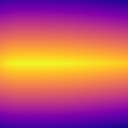
\includegraphics[width=0.8\linewidth]{statics/airfoil_sdf_high.png}
        \caption{SDF High}
      \end{figure}
    \end{column}
  \end{columns}
\end{frame}

\begin{frame}{Koreksi Bug Rotasi SDF Airfoil}
  Penggunaan argumen fungsi \texttt{warpAffine} di OpenCV sudah diperbaiki\footnote{\url{https://github.com/akbarpn136/aerofoil/pull/10/commits/6b2cbc11bf748381a9f6177456362794eb791a24}}.

   \begin{figure}[h]
    \centering
    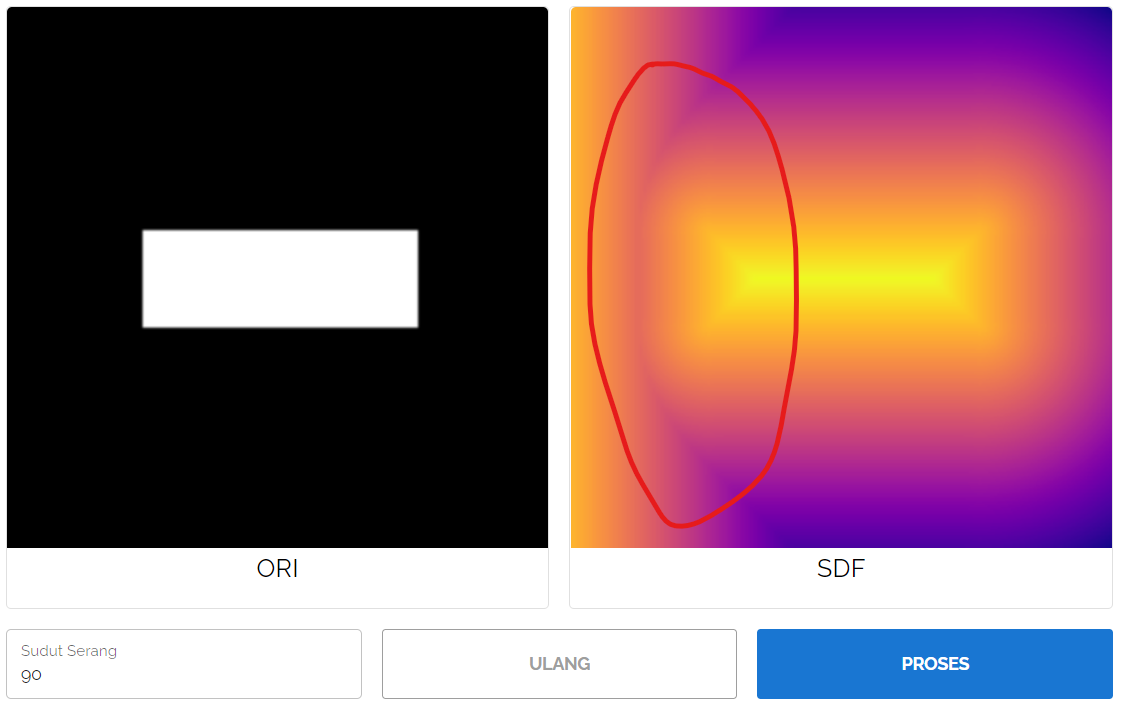
\includegraphics[width=0.5\linewidth]{statics/bug_rotasi}
    \caption{Setelah koreksi}
  \end{figure}
\end{frame}

\subsection{Telaah Literatur}

\begin{frame}{Literatur Berkaitan XFLR5}
  XFLR5 merupakan aplikasi perancangan dan analisis airfoil yang menggunakan kode basis dari XFOIl\footnote{\url{https://web.mit.edu/drela/Public/web/xfoil/}} untuk analisis dua dimensi performa aerodinamika airfoil \cite{guzelbey2018numerical}.\\~\\

  \pause

  XFOIL dijalankan melalui \texttt{CLI} di terminal sehingga berbasis teks, sedangkan XFLR5 memiliki \texttt{GUI}.\\~\\

  \pause

  XFLR5 dapat digunakan untuk menghitung koefisien aerodinamika pada airfoil seperti $C_l$, $C_d$, $C_m$ dan $C_p$ \cite{Deperrois2009}.
\end{frame}

\begin{frame}{Literatur Validasi XFLR5}
  XFLR5 sudah divalidasi melalui refrensi penelitian-penelitian yang dilakukan, diantaranya:
  \pause

  \begin{columns}[t]
    \begin{column}{.5\linewidth}
      \begin{figure}[h]
        \centering
        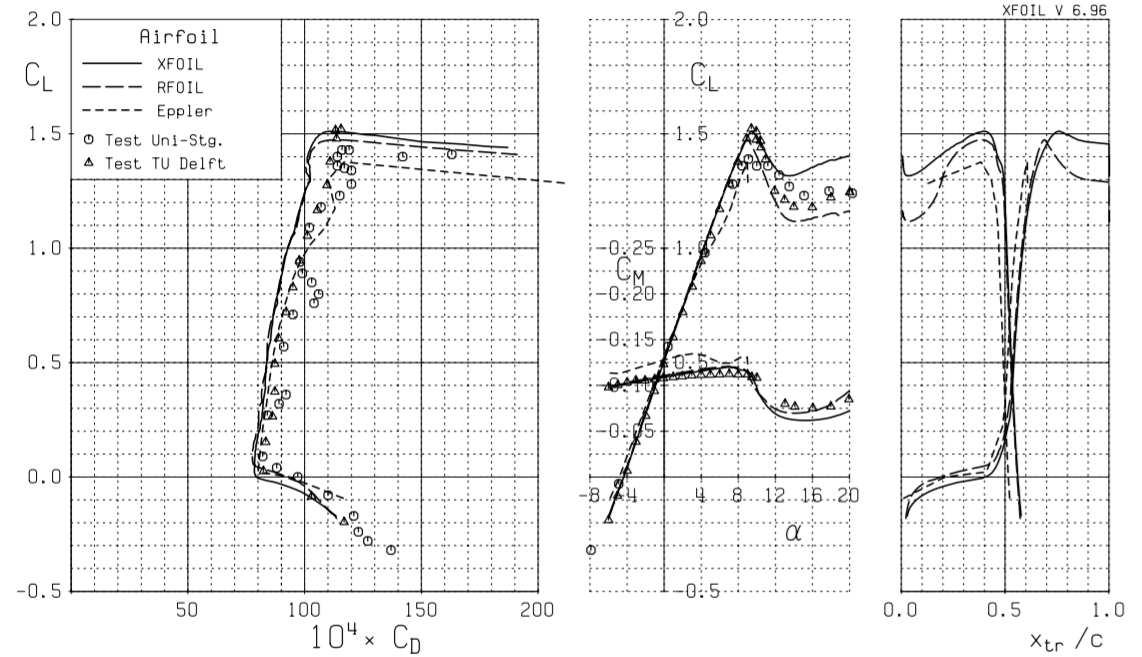
\includegraphics[width=0.8\linewidth]{statics/compar_airfoil1}
        \caption{Perbangingan data $C_l$}
        \label{fig:comparairfoil1}
      \end{figure}
    \end{column}

    \begin{column}{.5\linewidth}
      \begin{block}{\text{Analysis of three wing sections}}
        \cite{lasauskas2009analysis} melakukan perbandingan antara \texttt{XFOIL}, \texttt{RFOIL} dengan data pengujian terowongan angin di \textit{Stuttgart University} dan \textit{Delft University of Technology} dengan tingkat tubulensi rendah sekitar $0.04\:\%$.
      \end{block}
    \end{column}
  \end{columns}
\end{frame}

\begin{frame}{Literatur Validasi XFLR5 \textit{(lanjutan)}}
  \begin{columns}[t]
    \begin{column}{.5\linewidth}
      \begin{figure}[h]
        \centering
        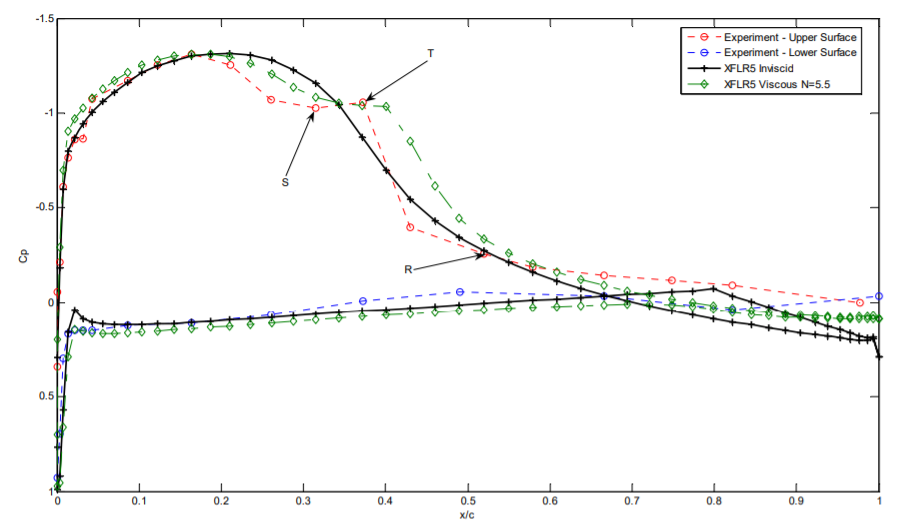
\includegraphics[width=0.8\linewidth]{statics/compar_airfoil2}
        \caption{Perbangingan data $C_p$}
        \label{fig:comparairfoil2}
      \end{figure}
    \end{column}

    \begin{column}{.5\linewidth}
      \begin{block}{\text{Experimental Investigation}}
        \cite{wahidi2009experimental} melakukan investigasi data pengujian terowongan angin dan kemudian dibandingkan dengan hasil kalkulasi \texttt{XFLR5}.\\~\\

        Kecocokan hasil $C_p$ pengujian terowongan angin dengan \texttt{XFLR5} dinilai baik.
      \end{block}
    \end{column}
  \end{columns}
\end{frame}

\begin{frame}{Literatur Validasi XFLR5 \textit{(lanjutan)}}
  \begin{columns}[t]
    \begin{column}{.5\linewidth}
      \begin{figure}[h]
        \centering
        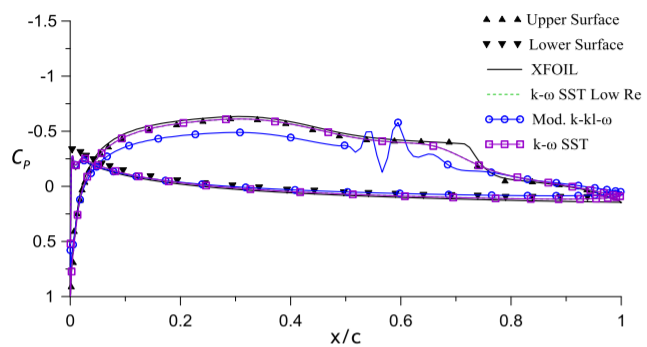
\includegraphics[width=0.8\linewidth]{statics/compar_airfoil3}
        \caption{Perbangingan data $C_p$ antar CFD}
        \label{fig:comparairfoil3}
      \end{figure}
    \end{column}

    \begin{column}{.5\linewidth}
      \begin{block}{\text{XFOIL vs CFD performance predictions}}
        \cite{morgado2016xfoil} Perbandingan antara data pengujian dengan prediksi dari \textit{solver CFD} lainnya, \texttt{XFOIL} tetap menjadi alat perancangan dan analisis airfoil yang baik.
      \end{block}
    \end{column}
  \end{columns}
\end{frame}

\begin{frame}{Uji Perbandingan}
  Melakukan perbandingan \texttt{XFLR5} dengan \texttt{airfoiltools}\footnote{\url{http://www.airfoiltools.com/airfoil/details?airfoil=n0009sm-il}}.\\~\\
  \pause

  Model airfoil \texttt{NACA 0009}.
  \pause

  \begin{columns}[t]
    \begin{column}{.33\linewidth}
      \begin{figure}[h]
        \centering
        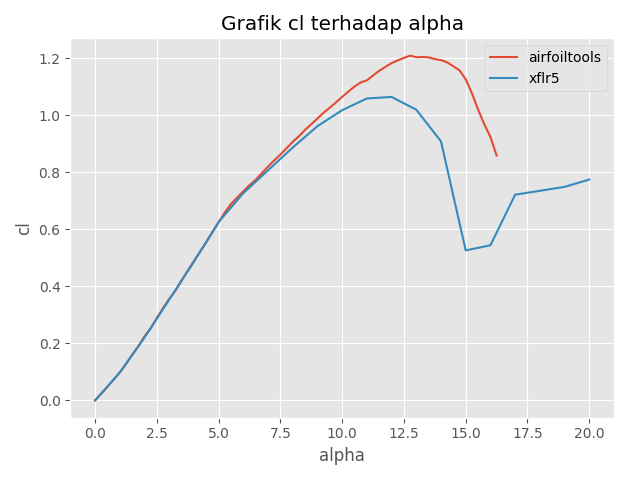
\includegraphics[width=0.8\linewidth]{statics/plot_naca0009_cla}
      \end{figure}
    \end{column}

    \begin{column}{.33\linewidth}
      \begin{figure}[h]
        \centering
        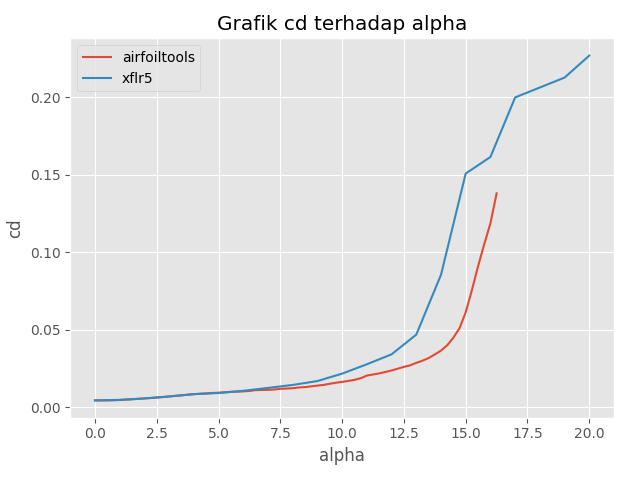
\includegraphics[width=0.8\linewidth]{statics/plot_naca0009_cda}
      \end{figure}
    \end{column}

    \begin{column}{.33\linewidth}
      \begin{figure}[h]
        \centering
        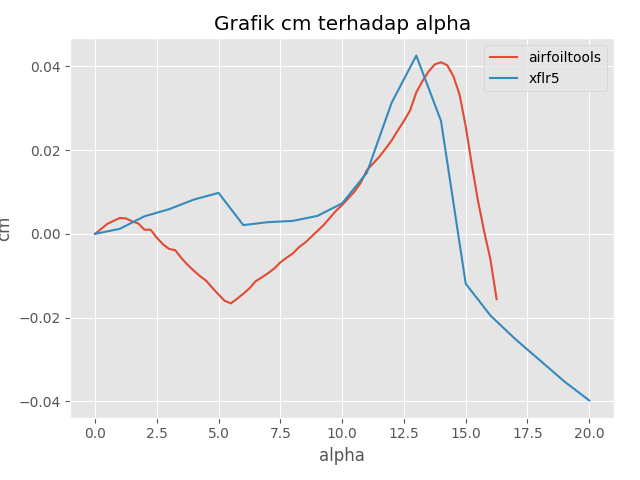
\includegraphics[width=0.8\linewidth]{statics/plot_naca0009_cma}
      \end{figure}
    \end{column}
  \end{columns}
\end{frame}
